\documentclass[onecolumn, 12pt]{article}

%!TeX spellcheck =fr
  \usepackage[utf8]{inputenc}
  \usepackage{hyperref}
  \usepackage[T1]{fontenc}
  \usepackage[francais]{babel}
  \usepackage{layout}
  \usepackage{verbatim}[4]
  \usepackage{color}

  \usepackage{graphicx}
  \usepackage{caption}
  \usepackage{subcaption}

  \usepackage{titlesec}

  \setcounter{secnumdepth}{4}

  \titleformat{\paragraph}
  {\normalfont\normalsize\bfseries}{\theparagraph}{1em}{}
  \titlespacing*{\paragraph}
  {0pt}{3.25ex plus 1ex minus .2ex}{1.5ex plus .2ex}


\title{Introduction au problème : le phénomène des Fake News.}
  \author{Enzo Poggio}
\begin{document}
\maketitle{}

%%%%%%%%%%%%%%%%%%%%%%%%%%%%%%%%%%%%%%%%%%%%%%%%%%%%%%%%%%%%%%%%%%
%%%%%%%% Part 1 Introduction au problème %%%%%%%%%%%%%%%%%%%%%%%%%
%%%%%%%%%%%%%%%%%%%%%%%%%%%%%%%%%%%%%%%%%%%%%%%%%%%%%%%%%%%%%%%%%%
\section{Qu'est-ce qu'une Fake News?}
\subsection{Définition d'une Fake News.}
\subsubsection{Produire des Fake News; une intention de tromper.}
%Distinguer les fake news des informations erronées dues à une erreur
%scientifique ou journalistique.

Un énoncé peut être vrai ou faux.
Il est vrai : s'il est en adéquation avec le monde.
Il est faux : s'il ne correspond pas à la réalité.
Les nouvelles (news) sont des énoncés.
Est-ce que l'énoncé \og J'aime les tartes. \fg  est une news ?
Non, toutes les news sont des énoncés; mais seul certains énoncés sont des news. Des journalistes ont fait une liste non exhaustive des critères d'une news (\href{http://www.tandfonline.com/doi/full/10.1080/1461670X.2016.1150193}{Tony Harcup et Deirdre O’Neill, 2016}).
La news est une histoire d'une personne de pouvoir ou célèbre.
Elle est parfois une bonne ou une mauvaise nouvelle.
Souvent elle est une surprise ou un phénomène qui concerne beaucoup de personnes.
Certaines sont juste des suivis, des divertissements ou des faits divers.
En somme, retenons qu'une nouvelle est une histoire en lien avec la réalité.
Ce qui nous intéresse c'est sa véracité selon l'interprétation du monde réel.
Cependant, leurs sujets sont variés, mais ce n'est pas pertinent pour nous.
De manière, plus générale une nouvelle est une histoire relayée par un média.

L'erreur est une opinion, un jugement ou une information non conforme avec la réalité ou la vérité.
L'erreur est inconsciente.
Elle n'est pas faite exprès.
Celle-ci démasquée, elle tend à être corrigée.
Une nouvelle erronée est donc une histoire médiatisée qui n'est pas vraie.
Elle ne correspond pas à la vérité.
La nouvelle erronée est due à une erreur scientifique ou bien une erreur journalistique.
C'est-à-dire une mauvaise manipulation de l'information par l'un de ces deux corps.
Les médias précautionneux corrigent leurs nouvelles erronées par des articles de démenti.
Ceci devrait être le code de déontologie des journalistes pour l'honnêteté intellectuelle.
Une Fake News\footnote{En français, nouvelle truquée mais le terme Fake News est devenu tellement commun
en français qu'il sera utilisé dans ce mémoire.} n'est pas une nouvelle erronée.
Cependant elles sont souvent confondues.

Parfois des nouvelles sont volontairement erronées.
On dit alors qu'elles sont fausses.
Il faut distinguer deux types de fausses nouvelles.
Le point important ici est l'intention derrière.

Les fausses nouvelles dans un but bien-veillant s'appellent satire ou information parodique.
Ces parodies imitent les médias.
Ils volent même jusqu'à leur nom parfois (le Gorafi est l'anagramme du Figaro).
Mais au lieu de diffuser de vraies informations, les parodies proposent un contenu décalé, sarcastique ou canularesque.
Le but premier de ce genre de nouvelle est le divertissement.
Même si l'on trompe le lecteur, on ne cherche pas à lui nuire mais plutôt à le faire rire.
Enfin il y a toujours des exceptions où l'information semble tellement crédible qu'elle est ensuite utilisée comme source fiable.
Les parodies donnent des informations délibérément fausses.
La tromperie est totalement assumée et même souvent revendiquée.

Les fausses nouvelles dans le but de volontairement tromper sont ce que l'on appelle Fake News.
Elle se distingue de l'erreur car elle n'est pas le produit du hasard ou d'une mauvaise manipulation.
Et elle se distingue de la satire et de la parodie car elle n'est ni assumée ni revendiquée fausse.
La Fake News provient d'un ensemble de médias.
Elle participe à la désinformation via les médias et les réseaux sociaux.
Souvent, les Fake News sont écrites par des anonymes difficilement contestables et calomniables.

\subsubsection{Limites de la définition.}
Certes une erreur peut arriver dans le traitement ou la création de l'information.
Mais ces erreurs sont-elles légitimes ?
La science progresse en faisant des erreurs.
D'ailleurs, dans la définition de l'étude scientifique l'erreur joue un rôle important.
L'étude scientifique est la recherche perpétuelle de l'erreur.
À défaut de nous apprendre ce qu'est la vérité, la science nous montre ce qu'elle n'est pas.
Donc l'erreur scientifique est légitime au bon fonctionnement de la science.
Peut-on en dire autant de l'erreur journalistique ?
Le journaliste doit faire un compte rendu exhaustif, objectif et vraisemblable du sujet qu'il traite.
Si une erreur non scientifique vient se faufiler dans son article c'est qu'il a mal fait son travail.

Par exemple, on voit toujours des médias relayer l'information que les vaccins causent l'autisme chez l'enfant.
Cette croyance persiste après une publication d'Andrew Wakefield
\footnote{Andrew Wakefield est un ancien chirurgien britannique et chercheur médical connu pour ses prétentions frauduleuses entre le vacin ROR et l'autisme.
Il fut radié de l'ordre des médecins en mai 2010 pour défaut à son devoir de consultant responsable.}.
Cette publication fut démentie des centaines de fois par des autorités compétentes, mais les médias de grande audience relayent toujours ce message de méfiance vaccinale.
Le devoir du journaliste n'est alors pas respecter .
Les médias traditionnels entretiennent le discours erroné des antivax
\footnote{Partisans de la controverse sur la vaccination qui remet en cause son efficacité et la sécurité de certains vaccins.}.
Celui-ci fait s'écouler beaucoup d'encre.
Mais cette controverse est de la désinformation pure et d'une grande malhonnêteté intellectuelle.


\subsection{Pourquoi produire des Fake News?}
\subsubsection{Le contexte des Fake News.}
%Dans une presse de plus en plus virtualisée chacun peut devenir l'auteur d'un article.
L'invention qui a le plus contribué à l'essor des médias est certainement l'imprimerie.
Elle nous fait passer des histoires orales à la presse.
L'information est figée sur du papier.
Elle n'est plus perdue ou transformée par le locuteur de l'histoire.
À partir de ces documents, on peut faire des versions officielles et approuvées par une autorité.
L'information fut pendant très longtemps partagée de manière verticale.
La source d'autorité de la connaissance était plus ou moins légitime et compétente.
La connaissance était donnée par les médias et leur vision. Il n'y avait pas de sources contestataires.

Puis fut créé internet ! Internet permet un partage des connaissances horizontal.
Tout le monde disposant d'une connexion au réseau peut participer à la connaissance générale.
Chacun peut écrire, partager et relayer des informations.
Les médias se sont développé sur internet et surtout ils s'y sont multipliés.
La pluralité du web qui permet de mieux recroiser ses sources.
Nous ne sommes plus dans la vision dogmatique des grands groupes qui possèdent les chaînes télévisuelles.

%La liberté d'expression d'internet permet certes de diffuser la connaissance mais aussi des inepties.
Nous avons acquis une énorme liberté d'expression avec l'avènement d'internet comme média souverain de la pluralité.
Mais ce nouveau régime pluriel a aussi des désavantages.
La démocratie de la connaissance permet aux profanes de s'exprimer sur des sujets de pointe.
Ainsi, nombreux sont les opinions et les préjugés qui sont travestis en pseudo-vérités.
La liberté d'expression et la facilité d'accès à internet participent grandement à la désinformation globale.

%Notre comportement face à internet = Knowing more and understanding less in the age of big data. (The internet of us Michael Patrick Lynch)
De plus la multiplicité qu'engendre internet pose un problème à notre compréhension du monde.
En effet comme le dit Michael Lynch, internet c'est \og connaître plus et comprendre moins [...]\fg
\footnote{Citation : \textit{Knowing more and understanding less in the age of big data} sous-titre du livre \textit{The internet of us}, de Michael Lynch ISBN-10: \href{https://www.kirkusreviews.com/book-reviews/michael-patrick-lynch/the-internet-of-us/}{0871406616}}.
M. Lynch conteste la notion largement acceptée qu'internet est un avantage parce qu'il rend plus d'informations disponibles à plus de gens plus rapidement et facilement.
\subsubsection{Le système monétaire des Fake News.}


%Explication rapide du clickbait.
Le clickbait désigne un contenu web qui vise à attirer le maximum de passages d'internautes afin de générer des revenus publicitaires en ligne.
Le clickbait affiche des gros titres racoleurs.
Il est souvent mensonger et sensationnel.
L'exactitude et les sources de l'article sont inexistantes.
Le but du clikbait est d'être partagé massivement sur les réseaux sociaux.

%Comment le clickbait est utilisé dans la presse actuelle ?
Maintenant que la presse virtuelle est multiple, pour être rentable, elle doit générer une offre publicitaire non négligeable.
Le clickbait est un effet pervers d'internet.
Les possesseurs de contenu peuvent gagner de l'argent par le biais de la publicité.
Cela crée des nouveaux systèmes monétaires.

%Les Fake news le premier client du clickbait.
Les Fake News et le clickbait associés répondent à la crise profonde de la presse papier au profit des réseaux sociaux comme médias.
De plus les Fake News alimentent une méfiance envers les médias traditionnels.
Elles font croire avec leurs \og faits alternatifs\fg qu'on tente de cacher quelque chose à la population.

\subsubsection{Raisons idéologiques.}
%Instrumentalisation de l'information pour servir un propos politique.
Les raisons idéologiques de produire des Fake News ne manquent pas.
En particulier en politique, où elles sont utilisées à tout va.
%Exemple Pizzagate Hillary Clinton
Un exemple probant est le Pizzagate.
En résumé le Pizzagate est une \og théorie\fg conspirationniste prétendant qu'il existe un réseau de pédophilie autour de John Podesta, l'ancien directeur de campagne d'Hillary Clinton.
Cette histoire fut rapidement démentie par les services de police et une majorité des médias américains. Mais les conséquences ne sont pas négligeables.
Un fusillade, heureusement sans blessé, a eu lieu dans la pizzeria où étaient soi-disant séquestrés les enfants du réseau pédophile de Podesta.


\subsection{Les origines des Fake News.}
\subsubsection{Des médias négligents.}
La négligence et l'unicité des médias fait que les Fake News peuvent se propager facilement.
Comme nous l'avons dit précédemment, les médias traditionnels traversent une crise.
La production de contenus doit être faites le plus rapidement possible.
Dans le but de répondre à la course à l'information de plus en plus grande et déloyale, la qualité des articles est revue à la baisse.
Certains journalistes ne font pas le travail de vérifier leurs sources pour accélérer le procédé de publication.



\subsubsection{Des organisations malveillantes internationales.}
L'appât du gain facile que sont les Fake News a suscité des vocations.
En Macédoine, une partie de la jeunesse de Vélès s'est ainsi spécialisée dans la création de Fake News, attirée par de juteux revenus publicitaires. La ville s'est transformée en fabrique à Fake News pendant l'élection américaine\footnote{D'après le \href{http://www.lefigaro.fr/actualite-france/2017/03/06/01016-20170306ARTFIG00187-fake-news-un-meme-terme-pour-plusieurs-realites.php}{Figaro} 20/12/2017 }.
Mais aussi des sites comme \href{https://www.infowars.com/}{InfoWars} voient naître des Fake News.

\begin{center}
 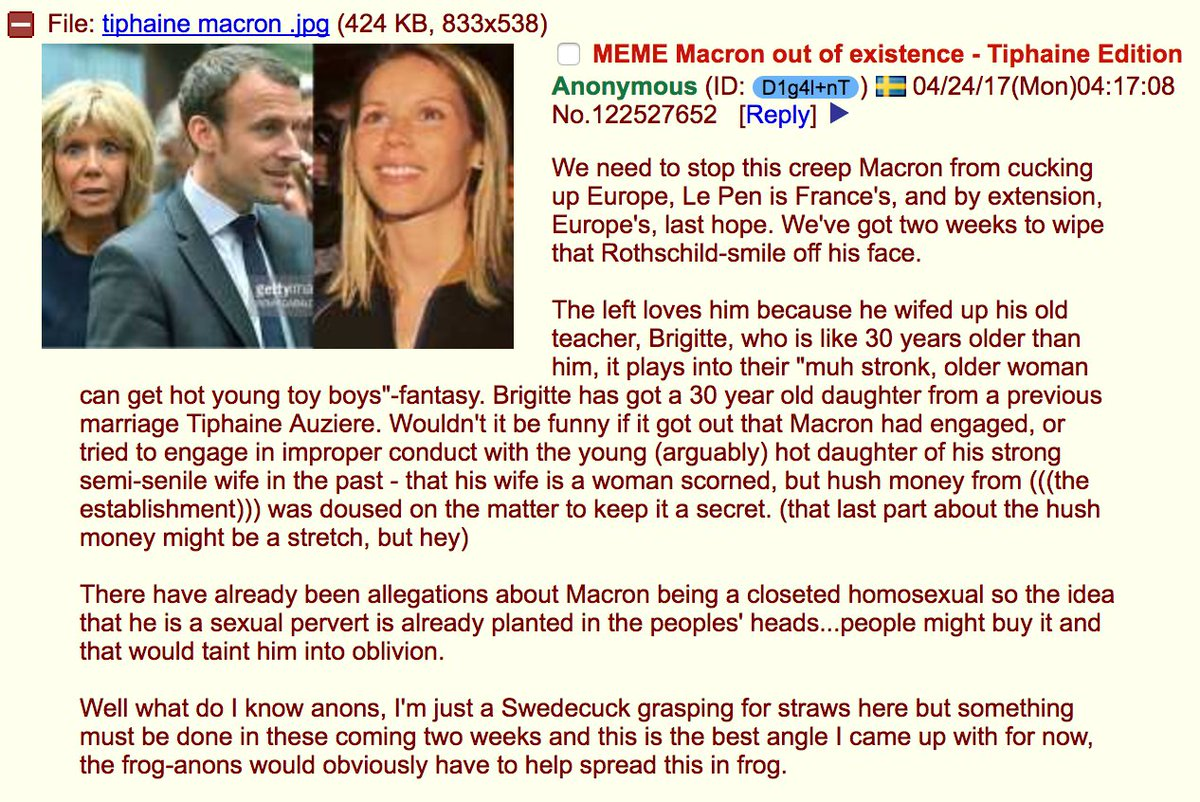
\includegraphics[scale=0.20]{../../img/rumeur_4chan/macron.jpg}
 \captionof{figure}{Capture d'écran d'un fil de discussion sur 4chan pour lancer une rumeur de pédophilie sur Macron.}
 \label{macron}
\end{center}

Des organisations qui travaillent dans l'ombre des plus grands forums sont à la base de la conception des Fake News.
En effet, l'étude de \href{https://arxiv.org/abs/1705.06947}{Savvas Zannettou et al, 2017} montre comment les forums leaders mondiaux que sont 4chan et reddit sont en partie responsable dans la création de rumeurs.


\subsection{La propagation des Fake News.}

\subsubsection{Les réseaux sociaux : médiations des Fakes News}
Selon \href{https://hal.inria.fr/hal-01281190}{Maksym Gabielkov et al, 2016}, 59\% des liens partagés sur Twitter n'ont jamais été cliqués.
En d'autres termes, la plupart des gens semblent retweeter des nouvelles sans jamais les lire.
Les personnes qui partagent sans lire des articles propagent certainement des Fake News sans le savoir.

Pour évaluer une Fake News nous n'avons pas besoin de dîplome.
En effet des études ont montré que les déterminismes sociaux n'étaient pas suffisants pour prévoir le partage de Fake News.
L'éducation, le sexe, l'âge, etc. ne sont pas des critères distinctifs.
\textcolor{red}{(Retrouver études...)}
Nous voyons alors que personne est à l'abri des Fake News. Seuls la pensée critique et le recul nous permettraient d'être protégés des Fake News.


\subsubsection{Le biais de confirmation.}
Les biais de confirmation sont un aspect déroutant de la pensée humaine.
Nous pourrions penser que l'homme ait acquis une pensée analytique développée pour arriver à ce niveau d'intelligence.
Et pourtant il est soumis au biais de confirmation.
Ce biais cognitif consiste à privilégier les informations confirmant nos idées préconçues ou nos hypothèses.
De plus il nous fait aussi négliger les informations jouant en défaveur de nos conceptions.

Ainsi les personnes tenantes de la thèse \og des extraterrestres gouvernent le pays\fg sont plus enclin à croire la thèse \og des reptiliens au pouvoir \fg que la thèse \og Barack Obama est un être humain \fg.

Les Fake News relayant souvent des informations conspirationnistes, il est facile pour un tenant de croire celle-ci plutôt que de croire des versions officielles.
Le biais de confirmation agit dans tous les sujets confondus. Il n'est pas uniquement cantonné au conspirationnisme. Les Fake News utilisent ce biais de manière idéologique pour renforcer nos croyances et nous rendre son information plausible.

\subsubsection{Tri de l'information selon Kahneman.}
La thèse centrale de Daniel Kahneman, dans son livre \og Système 1 / Système 2 : Les deux vitesses \fg, est qu'il y a une dichotomie entre deux modes de pensée.
Le système 1 est rapide, instinctif et émotionnel, alors que le système 2 est plus lent, plus réfléchi et plus logique.
Il définit les biais cognitifs associés à chacun de ces modes de pensée.
Il montre que l'on donne une trop grande importance au jugement humain.

Selon Kahneman nous nous reposons plus souvent sur le système 1.
Ce qui expliquerait notre partage de Fake News quand nous sommes émotionnellement impliqués.


\subsection{Les risques des Fake News.}
\subsubsection{Les risques politiques.}
%Comment les fakes news peuvent aider à cacher des scandales politiques.
L'institutionnalisation des Fake News est l'un des plus gros risques politiques.
En effet rien de pire qu'une Fake News qui a pour pseudo-autorité un état.
Un état niant les faits devient répressifs.
%Exemple les alternatives facts de l'institution de Donald Trump.
\begin{center}
 \begin{figure}[h]
  \begin{subfigure}{.5\textwidth}
   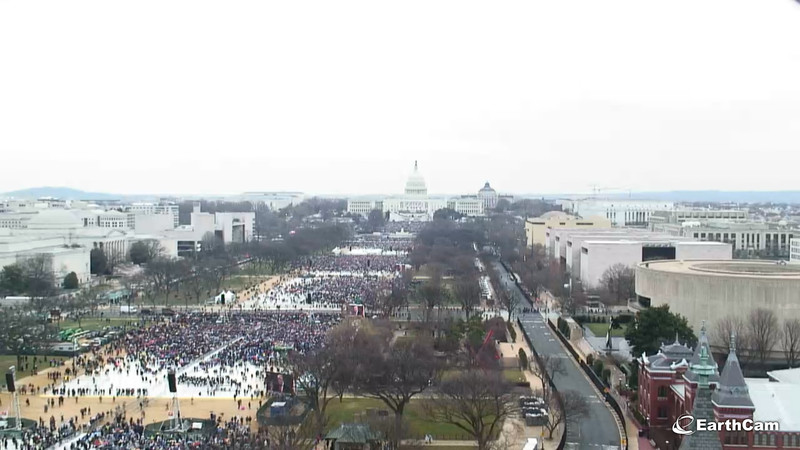
\includegraphics[scale=0.240]{../../img/trumpvswomen/trump.png}
   \caption{L'inauguration de Trump}
   \label{fig:sub1}
  \end{subfigure}
  \begin{subfigure}{.5\textwidth}
   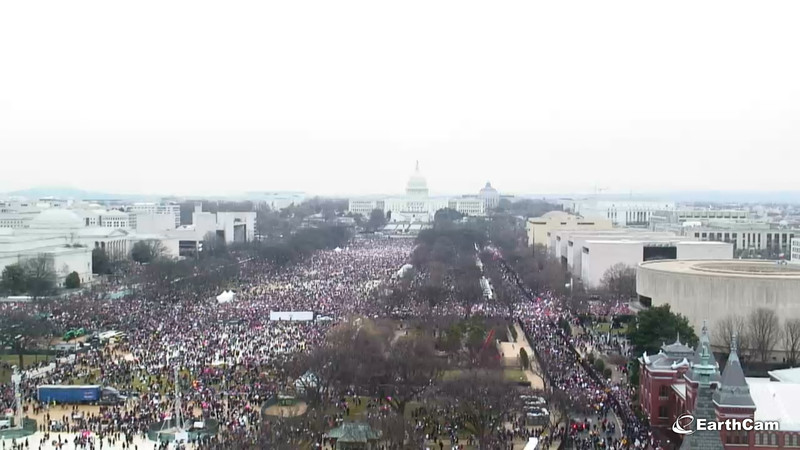
\includegraphics[scale=0.240]{../../img/trumpvswomen/women.png}
   \caption{Women’s March}
   \label{fig:sub2}
  \end{subfigure}
  \caption{Deux photos d'événements du National Mall à Washington}
  \label{fig:test}
 \end{figure}
\end{center}

L'inauguration de Trump et la Women's March avaient fait beaucoup de bruit.
Les partisans pro-Trump seraient soi-disant en plus grand nombre que les partisans de la Women's March.
Nous pourrions croire la version officielle.
Mais apparemment sans comptage, il y avait plus de participants à la Women's March.
L'État américain avaient tenté de faire passer cela pour des faits alternatifs.
Ce qui n'a pas beaucoup de sens.
Certes, nous observons tous le réel de manière différente, mais ce n'est pas une raison pour faire du relativisme et conclure à des faits alternatifs.
De plus comment définir des faits alternatifs ?
Prendre des faits et les dénaturer à des fins idéologiques ne nous donne pas raison sur la réalité.
En somme, les Fake News peuvent servir à cacher des scandales politiques.

D'autres Fake News institutionnalisées peuvent servir à des particuliers pour qu'ils puissent s'enrichir, ou à ne pas payer d'amende.
Par exemple, nier le réchauffement climatique est très pratique quand on est l'un des pays les plus polluant au monde.
\subsubsection{Les risques sanitaires.}
%Comment la santé peut être mise en danger par de fausse informations?
Beaucoup de Fake News portent sur les domaines sanitaires.
Comme nous l'avons vu précédemment avec les vaccins, les Fake News développent une méfiance pour la médecine conventionnelle.
Pour reprendre l'exemple des vaccins, il faut savoir que des cas de rougeole mortels sont réapparus ces dernières années. \textcolor{red}{(sources ?)}
Ne pas se vacciner entraîne un baisse de la couverture vaccinale.
Le rapport bénéfice/risque est plus que positif pour la vaccination.
Aucun des effets indésirables notoires suspectés n'a trouvé un protocole testable positif.
Nous n'avons que des affirmations pseudo-scientifiques et des hypothèses contre.
En somme, la désinformation, autour de la médecine notamment, peut couter la vie.

\subsubsection{Détournement des news vers des sujets clivants.}
Les Fake News peuvent être colportées par des personnes convaincues de leur véracité.
Le but ultime d'une Fake News est d'être considéré comme une vraie information.
Les Fake News détournent l'attention de la population vers des problèmes factices et souvent résolus depuis des années. En somme les Fake News sont une perte de temps. Elles nous empêchent de nous focaliser sur de vrais problèmes ; car l'on doit démystifier des faits irréels.

\subsection{Légitimité du projet et motivations.}
Comme nous avons pu le voir dans les sous-sections précédentes.
Les Fake News sont de fausses nouvelles qui cherchent à tromper volontairement.
Elles participent pour la majorité à une pollution du web dûe au système monétaire de la publicité en ligne.
Elles servent parfois un propos idéologique avec de mauvais argument.
Ceci les rend moins crédibles pour ceux qui découvrent le pot aux roses.
Elles sont produites par des militants anonymes anti-intellectuels prônant la désinformation sur de sombres forums.
Elles inondent les réseaux sociaux d'inepties et sont partagées en masse sans être lues.
Elles véhiculent des titres avec de fausses idées alors qu'un simple coup d'oeil au corps de l'article rend le propos infondé.
De plus,Elles coutent la vie à certains.
Et pour finir elles peuvent devenir un instrument politique redoutable et autoritaire.

Pour toutes ces raisons il est légitime de vouloir combattre le phénomène des Fake News.


\subsection{Comment détecter une Fake News?}

\subsubsection{Comment vérifier des informations ?}
%Exposer différentes méthodes pour les différents types de médias.
Il y a deux moyens de détecter une Fake News.
Par soi-même en cherchant les indices du canular.
Ou en utilisant un moteur de recherche de canular sur un domaine internet.

Premièrement voyons de manière non-exhaustive quelques techniques pour détecter une Fake News:
\begin{description}
 \item [Avant de partager] il faut se questionner sur ce qu'il est raconté dans l'article et vérifier les sources. On est responsable de ce que l'on partage.
 \item [Est-ce une information ?] Il faut se poser différentes questions: Est-ce cela à un intérêt public ? Est-ce factuel ? Est-ce vérifié ? Cela permet de distinguer les avis et les rumeurs des informations.
 \item [Ce site est-il fiable ?] A-t-il une page \og À propos \fg ? Est-il parodique ? Quelles sont les sources de ce site ?
\end{description}
Beaucoup de techniques spécifiques pour chaque média existent ! Nous ne pouvons pas être exhaustif ici.

Les Fake News ont fait apparaître de nouveaux sites spécialisés dans la détection de canulars.
Par exemple, en français, il existe le \href{http://www.lemonde.fr/verification/}{Décodex} propulsé par le journal le Monde. Ce site répertorie les autres sites selon leurs fiabilités.
En anglais il existe le site internet Polifacts de vérification des faits, qui vérifie la véracité des promesses et engagements pris par les politiques américains
%\paragraph{Les limites des MDR vérificateur de faits.}
%Premièrement passer des menottes au lieu d'ouvrir le débat n'est pas une bonne solution !

%Deuxièmement les conflits d'intérêts des grands groupes qui font du fact-checking n'est pas à négliger. Une source de connaissance univoque n'est pas objective.
\subsubsection{Méthode informatique: Stance detection.}
Cette tâche peut aussi être résolue avec un succès modeste par l'apprentissage automatique.
En effet une des réponses au phénomène des Fake News est l'apparition de réseaux neuronaux complexes qui permettent de manière partielle de repérer les Fake News. Ce repérage passe par une détection des partis pris (stance detection).

Ainsi dans la deuxième partie de ce mémoire, nous allons voir plus en détail ce qu'est la stance detection.
Au travers de tâches partagées, nous allons découvrir les techniques pour l'utiliser.

Dans la troisième partie nous nous essayerons à la Stance detection aussi.
Et donnerons une analyse comparative de nos résultats par rapport à l'état de l'art.

\end{document}
\grid
